\documentclass{article}

\usepackage[utf8]{inputenc}
\usepackage[T1]{fontenc}
\usepackage{graphicx}
\usepackage{amsmath}
\usepackage{amssymb}

\graphicspath{{./img/}}

%%%%%%%%%%%%%%%% Lengths %%%%%%%%%%%%%%%%
\setlength{\textwidth}{15.5cm}
\setlength{\evensidemargin}{0.5cm}
\setlength{\oddsidemargin}{0.5cm}
\setlength{\topmargin}{-2.5cm}
\setlength{\textheight}{24.5cm}

%%%%%%%%%%%%%%%% Variables %%%%%%%%%%%%%%%%
\def\projet{4}
\def\titre{Non-linear systems of equations / Newton-Raphson method }
\def\groupe{4}
\def\equipe{8631}
\def\responsible{ymougou}
\def\secretary{ilmourid}
\def\others{hpierre001, sabidi002, cpreaut}


%%%%%%%%%%%%%%%% Commands %%%%%%%%%%%%%%
\newcommand{\tvect}[2]{ \begin{pmatrix} #1 \\ #2 \end{pmatrix} }

\begin{document}

%%%%%%%%%%%%%%%% Header %%%%%%%%%%%%%%%%
\noindent\begin{minipage}{0.98\textwidth}
  \vskip 0mm
  \noindent
  { \begin{tabular}{p{7.5cm}}
      {\bfseries \sffamily
        Project \projet} \\ 
      {\itshape \titre}
    \end{tabular}}
  \hfill 
  \fbox{\begin{tabular}{l}
      {~\hfill \bfseries \sffamily Group \groupe\ - Team \equipe
        \hfill~} \\[2mm] 
      Manager : \responsible \\
      Secretary : \secretary \\
      Programmers : \others
    \end{tabular}}
  \vskip 4mm ~

  ~~~\parbox{0.95\textwidth}{\small \textit{Abstract~:} \sffamily This project is based on the development of an algorithm which can search the roots of a non-linear equation system. The method used is the Newton-Raphson algorithm and two examples were done to test this algorithm, the computation of the Lagrangian points and the search of electrostatics equilibrium.  Another algorithm was implemented to factorize polynoms with the Bairstow method. (\textit{Part written by Hugo PIERRE.})}
  \vskip 1mm ~
\end{minipage}

%%%%%%%%%%%%%%%% Main part %%%%%%%%%%%%%%%%
\section{Newton-Raphson algorithm} 

The Newton-Raphson algorithm requires the Jacobian matrix of the function so there were two options. The first one is to calculate the Jacobian matrix manually for each function processed by the Newton-Raphson algorithm and the second one is to write an algorithm that compute this matrix for a function given in parameter and a point where it is applied. \textit{Written by Hugo PIERRE.}\\

\subsection{Jacobian matrix}
\textit{Part written by Hugo PIERRE.}\\

This part deals with the algorithm that computes the Jacobian matrix. It uses the Taylor-Young formula to calculate partial derivatives discreetly. This algorithm was tested on a non-linear function:
\begin{equation}
  \label{eq:def_func_jacob}
  \begin{pmatrix}
    x \\
    y
  \end{pmatrix}
  \mapsto
  \begin{pmatrix}
    3xy \\
    x^2 \\
    4x(x+y)
  \end{pmatrix}
\end{equation}
The Figure 1  below represents the relative gap between the theoretical Jacobian matrix and the computed one for the function given by \eqref{eq:def_func_jacob}. The relative gap increases when the norm of $\tvect{x}{y}$ decreases, this is due to the fact that the parameter h is fixed in the algorithm but theoretically it has to be negligible compared to the norm of the vector in the Taylor-Young formula. Yet, as h is fixed, it is not negligible when x and y are closed to 0. However, because that way it could become negligible for the floating point calculation and thus lead the algorithm to be mistaken.

\begin{figure}[h]
  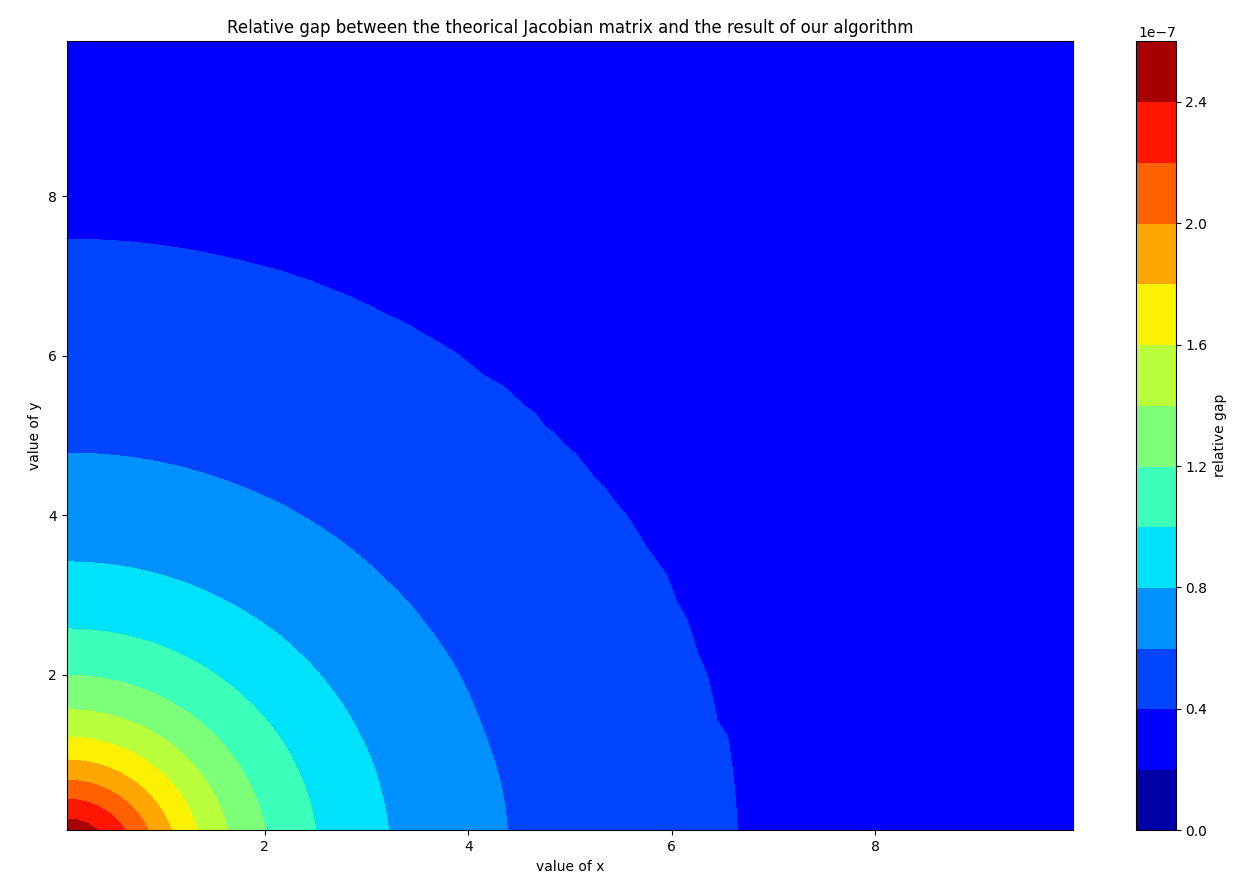
\includegraphics[scale=0.3]{rel_gap_jacob.png}
  \label{fig:rel_gap_jacob}
  \caption{Relative gap between theoretical and computed Jacobian matrix}
\end{figure}


\subsection{Newton-Raphson}
\textit{Part wrote by Clément PREAUT.}\\


\begin{figure}[h]
\begin{minipage}[c]{.3\linewidth}
    \centering
    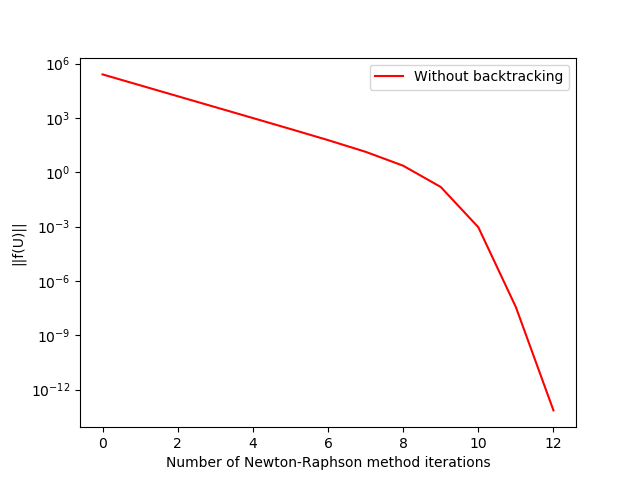
\includegraphics[scale=0.37]{Pictures/Newton_Raphson_pictures/R_to_R_tst.png}
    \caption{Primary test}
    \label{fig:R_to_R_tst}
\end{minipage}
\hfill%
\begin{minipage}[c]{.3\linewidth}
    \centering
    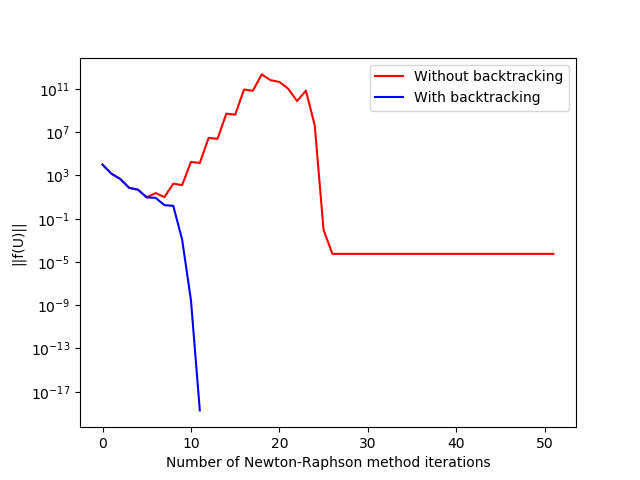
\includegraphics[scale=0.37]{Pictures/Newton_Raphson_pictures/Comp_back.png}
    \caption{Comparison with and without backtracking}
    \label{fig:Comp_back} 
\end{minipage}
\hfill%
\begin{minipage}[c]{.30\linewidth}
    \centering
    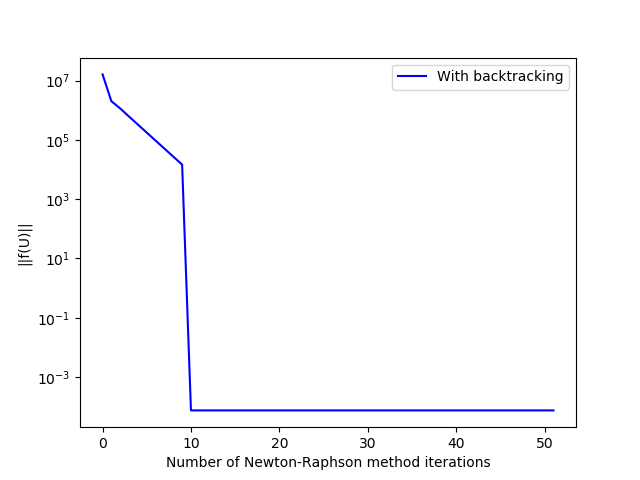
\includegraphics[scale=0.37]{Pictures/Newton_Raphson_pictures/extremum.png}
    \label{fig:extremum} 
    \caption{Extremum problem}
\end{minipage}
\end{figure}



In order to find a solution for $f(U) = 0$ for a given function f, the iterative Newton-Raphson method was used. For a given vector U , a function f and its associated Jacobian matrix H(U), a vector V was found so that $f(U + V) = 0$, where $f(U) + H(U) \times V$ approximated $f(U + V)$. This operation was reiterated until $||f(U)||$ was close enough to zero.
\\Therefore, in each iteration of the the \emph{Newton\_Raphson} function's \emph{while} loop, a new \emph{V} was found by solving $f(U) + H(U) \times V = 0$ thanks to \emph{numpy.linalg.lstsq} . The progress towards the desired result shifted from a linear speed to a quadratic speed below a level. 
\\In \emph{Figure} \ref{fig:R_to_R_tst}, the \emph{Newton\_Raphson} method was applied on the function :
\\$f : \mathbf{R} \longrightarrow \mathbf{R} , x \hookrightarrow x^2 + 3 \times x - 4$
\\The curve began to decrease dramatically after the breaking point of the tenth iteration. The function also returned value $||f(x)|| \simeq 7.10^{-14}$ and 1 for \emph{x}, which indeed belongs to the solutions.
\\Nevertheless, problems were encountered. In many cases the algorithm diverges. In consequence, initial conditions were chosen in an area in which a solution could be found. In addition, to avoid ifnite iterations of the algorithm, the implementaion could not execute more than an imposed number.
Moreover, in some circumstances, the norm of \emph{H(U)} was very low. It removed the vector \emph{V} far from the value of the vector \emph{U} therefore the relation $||f(U + V)|| \geq ||f(U)||$ risked to appear. Consequently \emph{Backtracking} consisted in reducing \emph{V} until the inequality inverted. In \emph{Figure} \ref{fig:Comp_back} above, applications of the \emph{Newton\_Raphson} method with and without backtracking were compared, on the function
\\$g : \mathbf{R}^2 \longrightarrow \mathbf{R}^2 , (x,y) \hookrightarrow (\frac{x + y}{x^2 + 1},(x^2 + 2) \times y)$.
\\First of all, with backtracking, the result constantly approached zero as well as in the first example, while without backtracking, the curve shot up until a peak of more than $10^{11}$. Finally, the intended result was obtained after the eleventh iteration thanks to backtracking whereas by applying the primal algorithm, the curve stayed at an unsatisfactory level until passing the limit number of iterations.
The main difficulty of the \emph{backtracking} method happened when \emph{U} was either a local minimum of a positive curve either a local minimum of a negative curve. The derivate oriented such that it made $||f(U)||$ the minimum value available near \emph{U}. Therefore, no vector \emph{V} added to \emph{U} and $||f(U)||$ thus remained steady. \emph{Figure} \ref{fig:extremum} above shows this.
Finally, by avoiding useless calls of \emph{numpy.linalg.norm} or \emph{f} when \emph{U} had not changed yet,the execution time was reduced.

\newpage
\section{Computation of the Lagrangian points}
\textit{Part written by Ibrahim LMOURID.}\\
Euler and Lagrange proved the existence of five equilibrium points in the restricted problem of the three bodies. Each point represents a position of space in a 2-body system (the Sun and the Earth for example), where their fields of gravity combine to provide an equilibrium point for a third body of negligible mass (satellite for example). Those points are commonly called: L1, ..., L5.

\subsection{Forces}
\noindent The goal of this section is to write the code of three kinds of forces: 
\begin{enumerate}
    \item An elastic force: \textbf{fe :}
    $\begin{pmatrix} 
    x \\ 
    y 
    \end{pmatrix}$ $\longrightarrow$
    $\begin{pmatrix}
    -k\times x \\
    -k\times y
    \end{pmatrix}$
    \item A centrifugal force: \textbf{fc :}
    $\begin{pmatrix} 
    x \\ 
    y 
    \end{pmatrix}$ $\longrightarrow$
    $\begin{pmatrix}
    k\times (x-x_0) \\
    k\times (y-y_0)
    \end{pmatrix}$
    
    \item A gravitational force: \textbf{fg :} 
    $\begin{pmatrix} 
    x \\ 
    y 
    \end{pmatrix}$ $\longrightarrow$
    $\begin{pmatrix}
    \frac{-k\times (x-x_0)}{((x-x_0)^2+(y-y_0)^2)^\frac{3}{2}} \\
    \frac{-k\times (y-y_0)}{((x-x_0)^2+(y-y_0)^2)^\frac{3}{2}}
    \end{pmatrix}$
\end{enumerate}
In order to represent these functions, three main algorithms were implemented:

\begin{enumerate}
    \item \textbf{elastic\_force}
    \item \textbf{centrifugal\_force}
    \item \textbf{gravitational\_force}
\end{enumerate}
Each of these cases needs two parameters:
\begin{enumerate}
    \item k : The intensity of the force
    \item ($x_{0}$, $y_0$) : A central point from which the force is issued.
\end{enumerate}
\subsection{Equilibrium points}
The goal of this section is to use the Newton\_Raphson algorithm to obtain the 5 Lagrangian points of an object moving in the plane and subject to these forces: 
\begin{enumerate}
    \item Gravitational force of the Sun, which was subject to: k=1 and $x_0$=0 and $y_0$=0.
    
    \item Gravitational force of the Earth, which was subject to: k=0.01 and $x_0$=1 and $y_0$=0.
    \item Centrifugal force centered on the barycenter of Sun and Earth, which was subject to: k=1 and $x_0$=0.01/1.01 and $y_0$=0.
\end{enumerate}
% Thus, it is necessary to change the vector U 0 and to apply again Newton_Raphson algorithm in order to obtain another equilibrium point. However, it’s possible to find the same equilibrium points, with the new vector U 0 . That’s why, it’s very important to apply the Newton_Raphson algorithm on a very large number of vectors. This approach allows us to find all Lagrangian points
The application of the Newton\_Raphson algorithm on a vector $U_0$(x,y) yielded a single equilibrium point. Thus, it was necessary to change the vector $U_0$ and to apply again the Newton\_Raphson algorithm in order to obtain another equilibrium point, with the new vector $U_0$. However, it was possible to find the same equilibrium point, with the new vector $U_0$. Consequently, it was very important to apply the Newton\_Raphson algorithm on a very large number  of vectors. This approach made it possible to find all Langrangian points.
\newline
It was decided to apply Newton\_Raphson algorithm on 1600 vectors, belonging to $[-5, 5]\times[-5, 5]$.
\newline
The graph in \textit{Figure 5} below  shows the results given by the algorithm \textbf{Lagrangian\_points()}: 
\begin{figure}
    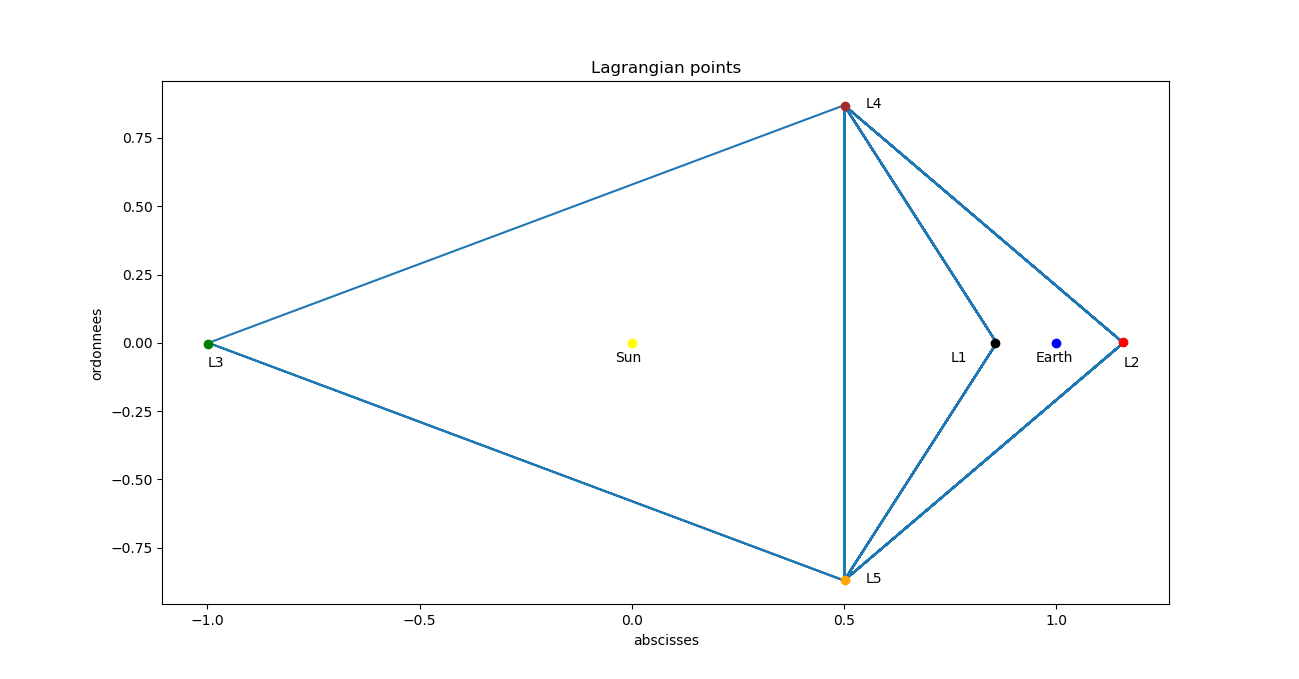
\includegraphics[scale=0.5]{./Pictures/Lagrangian/Figure_1-8.png}
    \caption{Lagrangian points}
    %\label{figure_1-6}
\end{figure}

\section{Electrostatic equilibrium}
\textit{Part written by Yassine MOUGOU.}\\

This section deals with the calculation of the total energy of a \emph{N}-charge system, provided that each charge is in circulation over the interval $[-1,1]$, and to find the equilibrium position for this system.\\
\begin{itemize}
\item[*]The total energy of the system is given by \eqref{Total_Energy}:\\
\end{itemize}
\begin{equation}
  E(x_1,...,x_N)=\sum^{N}_{i=1} (log|x_i+1| + log|x_i-1|+\frac{1}{2}\sum^{N}_{j=1,j\ne{i}}log|x_i-x_j|)
\label{Total_Energy}
\end{equation}
where:
\begin{equation*}
  x_i:position\ of\ the\ charge\ i\ \forall i \in {1,2,...,N}\
\end{equation*}
\begin{equation*}
 E:Total\ energy
\end{equation*}
\begin{itemize}
\item[*]Now let's move to our main aim which is the equilibrium position(maximum or minimum). Our method consists in calculating the gradient of the system's total energy and looking for a vector $U=(x_1,x_2,...,x_N)$ that makes that gradient null.
\item[-]In order to calculate $\nabla E(x_1,x_2,...x_N)$, the function \emph{\textbf{gradient\_elec\_energy}} has been used. It takes a vector \emph{x} as a parameter and returns a vector that represents \emph{$\nabla E(x)$} such as $x=(x_1,x_2,...x_N)$:
\end{itemize}
\begin{equation}
  \nabla E(x)=\sum_{j=1,j\ne{i}}^{N}\frac{1}{x_i-x_j} + \frac{1}{x_i-1} +\frac{1}{x_i+1} 
\end{equation}
After that, the function \emph{\textbf{gradient\_jacob}} was used and returns the Jacobian matrix:\\
\begin{equation}
    \left \{
   \begin{array}{l l l l}
     jacob_{i,j}   & = & \sum_{j=1,j\ne{i}}^{N}\frac{-1}{(x_i-x_j)^2} + \frac{-1}{(x_i+1)^2} + \frac{-1}{(x_i-1)^2} & \forall i=j\\
     jacob_{i,j}  & = & \frac{1}{(x_i+x_j)^2} & \forall i\ne{j}\\
   \end{array}
   \right .
\end{equation}
\begin{itemize}
\item[-]Unfortunately, our goal has not yet been reached. The existence of an equilibrium position had to be proved. This is why the function \emph{\textbf{Newton\_Raphson\_back\_modif}} was used. It takes the function \emph{f} as a parameter, its Jacobian matrix \emph{J}, the starting point \emph{U0}, max iterations count \emph{N} and finally the precision \emph{eps}, and provides us with two lists \emph{\textbf{iteration}} and \emph{\textbf{norme\_f}}.
\item[-]This function is an ideal application for our problem. \texttt{f} and \texttt{J} need to be chosen by this way: \emph{f} = \emph{\textbf{gradient\_elec\_energy}} and \emph{J} = \emph{\textbf{gradient\_jacob}} and as it can be seen in Figure \ref{blabla} below.
\end{itemize}
\begin{figure}[h]
  \begin{minipage}[c]{0.46\linewidth}
    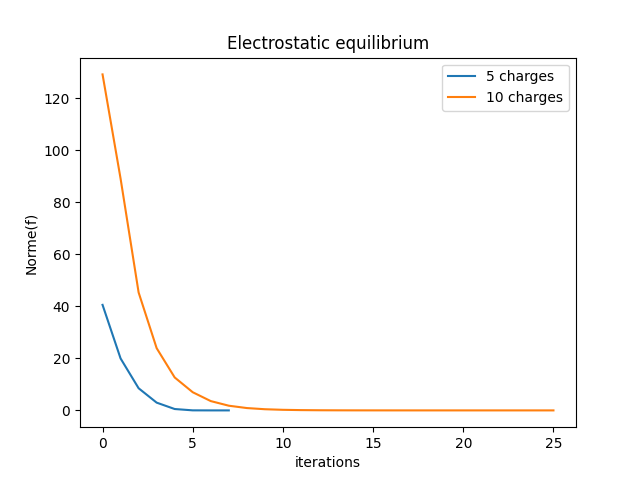
\includegraphics[scale=0.5]{Figure_2.png}
    \caption{Changes of $||\nabla E(x)||$}
    \label{blabla}
  \end{minipage}
  \hfill
  \begin{minipage}[c]{0.46\linewidth}
  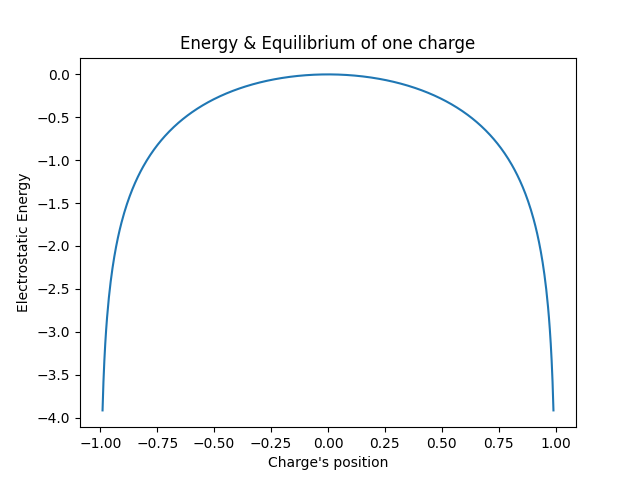
\includegraphics[scale=0.5]{Figure_1.png}
  \caption{Changes of the energy}
  \label{blablabus}
  \end{minipage}
\end{figure}
\subsection*{NB:}
\begin{itemize}
\item[*]There is an Electrostatic equilibrium because $||\nabla E(x)||$ converges to 0.
  \item[*]For Figure \ref{blabla} above, the Newton\_Raphson method with the backtracking was used and even if the Newton\_Raphson method was applied it would roughly lead to the same result. 
\end{itemize}
\begin{itemize}
\item[**]As it can be seen above, the existence of an equilibrium position was proved. Now it's time to check weather it is a maximum or minimum. 
\end{itemize}
\begin{itemize}
\item[**]According to Figure \ref{blablabus} above, the equilibrium position is a \emph{\textbf{maximum}} reached when $x=x1=0$.
\end{itemize}



\section{Bairstow method for polynomial factorization}
\textit{Part written by Saad ABIDI.}\\

To find the roots of a polynomial P the Newton \& Raphson method is valid, but only if it has real roots, which is not always the case. For this the Bairstow method is called, which searches for quadratic factors. The advantage of looking for quadratic factors is that it avoids any complex arithmetic.
The method consists in taking the polynomial in question and dividing it by a quadratic factor: 
\begin{equation}
    P(X)=(X^2 + BX + C)*Q(X)+RX+S \quad (B, C, R , S)   \varepsilon \mathbb{R} 
\end{equation}
Given B and C, R and S can be readily found.Therefore it can be said that R and S are functions of B and C,and they are nil if the quadratic factor is a divisor of P(X).
The aim was to find where (B,C) are simultaneously roots of R and S with the Newton \& Raphson method.\\
In other words Newton \& Raphson's method have to be applied on the function which takes as its parameter B C and returns R (B, C) and S (B, C).
Then the Jacobian matrix had to be determined,it represents the matrix of the partial derivatives of R and S compared to B and C. This matrix is calculated from a second division of Q by the quadratic factor.
By finding this ,the Newton\&Raphson function could be applied to find where (R,S)=(0,0).\\
\begin{figure}[h]
  \centering
  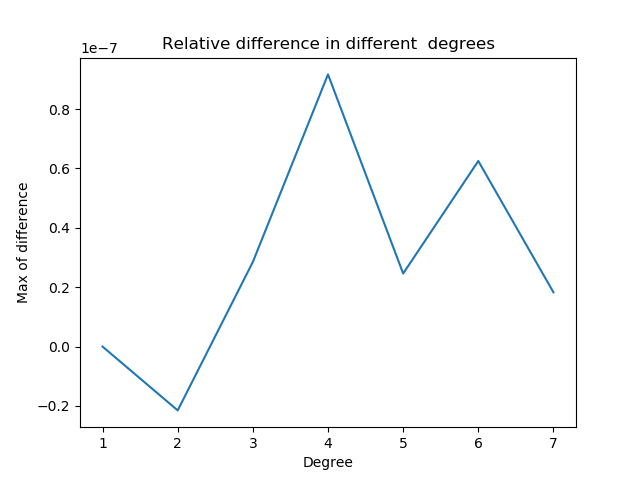
\includegraphics[scale=0.5]{Bairstow.png}
  \caption{Relative difference in different degrees}
  \label{fig:gg}
\end{figure}
After that the roots of the quadratic factor were found, and the same operation was repeated for the polynomial Q until a second order polynomial was obtained.\\
To test our function the Bairstow method was applied to several polynomial generated randomly in order to see the difference between the roots of this polynomial obtained through our method and those provided by the np.roots function .
Based on that a graph was generated to show the maximum relative difference in each degree between the two methods :\\
The graph \ref{fig:gg} above shows that the difference between the two methods fluctuate around $ 10^{-7}$
and that's what makes the Bairstow method efficient.

\subsection{Conclusion}
\textit{Part written by Hugo PIERRE.}\\

To conclude, this project leaded us to work in group and share the work. Moreover it make us discover the Newton-Raphson method which is efficient to find roots of non-linear equations system but one starting vector lead to one root so if there are many roots it demands to think the value of this vector for each root in order find them all. However this method is limited for many particular cases.

\end{document}
